% Created 2023-02-21 Tue 20:08
% Intended LaTeX compiler: pdflatex
\documentclass[final, 12pt] {ubb_dolgozat}{book}
\usepackage[utf8]{inputenc}
\usepackage[T1]{fontenc}
\usepackage{graphicx}
\usepackage{longtable}
\usepackage{wrapfig}
\usepackage{rotating}
\usepackage[normalem]{ulem}
\usepackage{amsmath}
\usepackage{amssymb}
\usepackage{capt-of}
\usepackage{hyperref}
\usepackage{minted}
\submityear{2022}
\doctypeHU{Szakdolgozat}
\doctypeEN{Diploma Thesis}
\doctypeRO{Lucrare de licenta}
\specHU{Informatika}
\specEN{Computer Science}
\specRO{Informatică}
\titleHU{Szakdolgozat cím}
\titleEN{License thesis title}
\titleRO{Titlu lucrare licență}
\authorHU{Zediu Álmos-Ágoston}
\authorRO{Álmos-Ágoston Zediu}
\authorEN{Álmos-Ágoston Zediu}
\tutorHU{dr. Bodó Zalán}
\tutorRO{dr. Bodó Zalán}
\tutorEN{dr. Bodó Zalán}
\pagenumbering{gobble}
\author{Álmos-Ágoston Zediu}
\date{\today}
\title{Szakdolgozat}
\hypersetup{
 pdfauthor={Álmos-Ágoston Zediu},
 pdftitle={Szakdolgozat},
 pdfkeywords={},
 pdfsubject={},
 pdfcreator={Emacs 28.2 (Org mode 9.6)}, 
 pdflang={English}}
\usepackage{natbib}
\begin{document}

\maketitle
\tableofcontents


\chapter{Bevezetés}
\label{sec:orge75e293}
\chapter{Technológiai alapok}
\label{sec:org6631bef}
\section{Clojure}
\label{sec:org676d80f}
A Clojure programozási nyelv egy dinamikus funkcionális nyelv, mely ötvözi a JVM platform előnyeit a Lisp nyelvek
kifejezőkészségével.
\subsection{Funkcionális programozás Clojureben}
\label{sec:orgad2e12f}

A Clojureben a függvények az elsőrendű absztrakciók, képesek vagyunk akár argumentumként is kezelni őket, stb.

\begin{minted}[]{clojure}
(defn my-adder [a b]
  (+ a b))

(def my-five-adder (partial my-adder 3))
(map my-five-adder [1, 2, 3, 4])
\end{minted}

\begin{itemize}
\item (``\#'user/my-adder'')
\item (``\#'user/my-five-adder'')
\item (``(4 5 6 7)'')
\end{itemize}

\subsection{Perzisztens adatstruktúrák}
\label{sec:org27c12b4}
Rich Hickey az adatstruktúráit az ideális hasítófákra alapozta \citep{bagwellIdealHashTrees2001}. Egy konceptuális elképzelésért
rátekinthetünk erre a képre:

\begin{center}
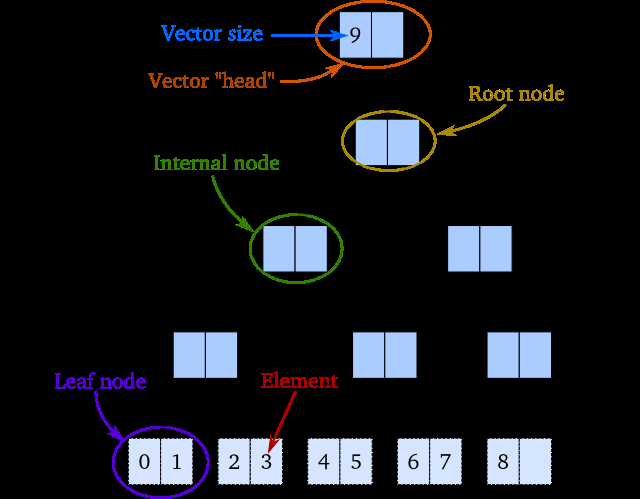
\includegraphics[width=.9\linewidth]{images/perzisztens-vektor.jpg}
\end{center}

A lényegi rész az, hogy ahhoz, hogy olyan adatstruktúrák, mint a vektorok performánsak legyenek, de perzisztensek, szükségünk van
specializált bináris fák felépítésére.
\chapter{Algoritmusok}
\label{sec:org32b5602}
\section{Locality sensitive hashing}
\label{sec:org54a0d69}
Lehet beszélni erről a \citep{charikarSimilarityEstimationTechniques}, vagy pedig,

\section{SVD}
\label{sec:org9b2edd9}
\citep{brandFastOnlineSVD2003}

\bibliographystyle{./abbrvnat_hu.bst}
\bibliography{/home/hrothgar32/Documents/Egyetem/Allamvizsga/Dolgozat/allamvizsga,/home/hrothgar32/Documents/allamvizsga/allamvizsga}
\end{document}